\documentclass{article}

\usepackage{booktabs} % for toprule, midrule, bottomrule in tables
\usepackage{authblk} % for multiple authors and affiliations
\usepackage{graphicx} % to inlcude graphics with \includegraphics
\usepackage{setspace}
\usepackage[a4paper, total={5.5in, 7.5in}]{geometry}
\usepackage{sectsty}
\usepackage{parskip}
\usepackage{xcolor}
\usepackage{booktabs}
\usepackage{subcaption}
\usepackage{listings}
\usepackage{tcolorbox}
\usepackage{amssymb}
\tcbuselibrary{theorems}
\newtcbtheorem
  []% init options
  {definition}% name
  {Definition}% title
  {%
    breakable,
    colback=white,
    colframe=blue!25,
    fonttitle=\bfseries,
    coltitle=black,
    boxed title style={
    sharp corners,
    size=small,
    colback=blue!25,
    colframe=blue!25,
    }
  }% options
  {def}% prefix

\newtcbtheorem
  []% init options
  {theorem}% name
  {Theorem}% title
  {%
    breakable,
    colback=white,
    colframe=gray!25,
    fonttitle=\bfseries,
    coltitle=black,
    boxed title style={
    sharp corners,
    size=small,
    colback=gray!25,
    colframe=gray!25,
    }
  }% options
  {theo}% prefix

\subsectionfont{\normalfont\itshape}
\subsubsectionfont{\normalfont\itshape}
%\usepackage{nameref}
%\usepackage{blindtext}
%\usepackage{subcaption}
\usepackage[toc,page]{appendix}
%\usepackage{multirow}
%\usepackage[linesnumbered,ruled]{algorithm2e}
\usepackage{url}
%\usepackage{algorithmic}
%\usepackage{algpseudocode}
%\usepackage{algorithm}
%\usepackage{hyperref}
\usepackage[utf8]{inputenc}
\usepackage{amssymb}
%\setlength\parindent{0pt}
\usepackage{mathtools}
\usepackage{amsmath}
\usepackage{hyperref}
\usepackage{amsthm}
%\usepackage{ragged2e}
\usepackage{natbib}
\usepackage{float}
\usepackage[ddmmyyyy]{datetime}
%\newdate{date}{31}{03}{2022}
\date{\displaydate{date}}
%\setlength\parindent{0pt}


\author[1]{Claudia Viaro}
%\affil[1]{First author's affiliation}


\title{Deep optimal switching\\[1ex]

\large{Approximating the indicator function with NN}}

\begin{document}

\maketitle
\displaydate{}
\setstretch{1.25}
%\doublespacing
%\onehalfspacing
%\begin{abstract}
%    Abstract 
%\end{abstract}
%\newpage

%\newpageremove date from oe
\tableofcontents
\newpage
%-------------------------------------------------------------
\section{Introduction}
An updated record of the implementations produced can be found at the following link \href{https://github.com/claudia-viaro/optimal_switching}{Optimal Switching}.


\section{Optimal stopping problems} \label{OptStop}
The treatment of a sequential decision making setting can be looked at from a more established and traditional perspective, that of an optimal stopping problem. We are interested in finding an optimal control policy that determines when to perform an intervention, given some observed characteristics, so as to maximize the expected total discounted return. It is clear that the problem at hand belong once again to the general class of Markov Decision Processes (MDP). 

\medskip
Fields of application largely include financial strategies (asset selling, hedging) but also sequential hypothesis testing. This topic is also relevant for healthcare applications such as in \cite{ajdari2019towards}, in determining when to stop the treatment of patients receiving fractionated radiotherapy treatments. Some applications also feature handling of engagement platforms \citep{liyanage2019automating}. 

\begin{definition}{Optimal stopping}{}
Let $(\Omega, \mathbb{F} = (\mathcal{F})_{n=0}^N, \mathbb{P})$ be a complete probability space, with $N \in \mathbb{N}$ be a natural number. Consider the time discretization with equidistant time grid $t_0, t_1, \ldots, t_N \in [0, T]$ and $0 = t_0 < t_1 < \cdot < t_N = T$. The discretization allows for a few simplifications involving the use of simpler algorithms for dicrete-state MDP (as opposed to semi/continuous MDP) as well as simplifications regarding the computation of one-step conditional expectations. \\
Let a $d$-dimensional discrete-time Markov process describe the asset price under a Black-Scholes market $(X_{t_n})_{n=0}^N$ with $X_0=x_0$ and be defined on the probability space given:
\begin{equation}\label{eq:eq1}
    X_{t}^i = (r-\delta_i)d t + \sigma_i d W_t^i
\end{equation}
where $r \in [0, \infty]$ is the market risk free rate, $\delta_i \in [0, \infty]$ is the dividend yield, $\sigma_i \in [0, \infty]$ is the volatility and $W: [0, T] \times \Omega \rightarrow \mathbb{R}^d$ be a standard Brownian motion on the same probability space, with $i=1, \ldots, d$ stock prices. \\
Call a random variable $\tau: \Omega \rightarrow \{ t_0, t_1, \ldots, t_N \}$ an $X$-stopping time if $\{\tau = n  \} \in \mathcal{F}$. The notion of reward (hence the price) we seek to maximize is: 
\begin{equation}\label{eq:eq2}
    V = \sup_{\tau \in \mathcal{T}} \mathbb{E} [g(\tau, X_{\tau})]
\end{equation}
where $\mathcal{T}_n$ denotes the family of all stopping times and $g(n, X_{t_n})$ is the discounted payoff process.\\
\end{definition}

The problem is then a Markov decision process with state space $\mathcal{S} = \{ 0, 1, \ldots, N \} \times \mathbb{R}^d \times \{0, 1 \}$, binary action space $\mathcal{A}= \{0, 1 \}$, where $a=0$ stands for holding on the option and $a=1$ for stopping the process (e.g. exercising the option) and reward function
\begin{equation}\label{eq:eq3}
    R((n, X_{t_n}), a)=
    \begin{cases}
      g(n, X_{t_n}) & \text{if } $a=1$\\
      0 & \text{if } $a=0$
    \end{cases} 
\end{equation}
for $n=0, \ldots, N$, transition kernel $p$ induced by the dynamics of the $\mathbb{F}$-Markovian process $(X_{t_n})_{n=0}^N$. The state space includes time, the $d$-dimensional Markovian process and an absorbing state that captures the event of exercising or not the option, as we do not consider repeated controls.

\smallskip
If perfect knowledge of the MDP is assumed and its size is limited, optimal stopping problems with finitely many stopping opportunities can be solved exactly, such as with backward induction on binomial/trinomial trees or lattice. It is in fact known that the Snell envelope $V^{\ast}$ provides an optimal solution to \ref{eq:eq2} \citep{peskir2006optimal}:

\begin{equation}\label{eq:eq4}
\begin{split}
   &U_N := g(X_N),\\
   &U_n := \max (g(X_n), \mathbb{E}[\alpha U_{n+1} | X_n]),
\end{split}   
\end{equation}
where $\alpha$ is a discount factor. Equivalently, $U_n$ can be expressed as the optimal stopping problem of the form:
\begin{equation}\label{eq:eq5}
   U_n = \sup_{\tau \in \mathcal{T}_n} \mathbf{E}[\alpha^{\tau - n}g(X_{\tau}| X_n)]
\end{equation}
where $\mathcal{T}_n$ is the set of all stopping times $\tau \leq n$. The associated optimal stopping time $\tau^{\ast}$ is the first time the immediate reward dominates the continuation value:
\begin{equation}\label{eq:eq6}
\begin{split}
&\tau_N := N,\\
&\tau_n := \begin{cases} 
n, & \mbox{if } g(X_n) \geq \mathbb{E}[\alpha U_{n+1}| X_n] \\ 
\tau_{n+1}, & \mbox{otherwise.}  \end{cases}
\end{split}
\end{equation}

On the other hand, when the state space is large (e.g. when the payoff depends on several underlying assets or when the payoff depends on the history of underlying’s prices), the classical algorithms used in the mathematical finance for exotic derivative pricing are no longer computationally tractable. Several approximations methods have been studied in the context of American/Bermudan option pricing, from approximation of the Snell envelope or continuation values \citep{longstaff2001valuing, carriere1996valuation}, to dual methods \citep{haugh2004pricing}. More recently, numerical approximation methods that are based on deep learning have been exploited. 

\subsection{Approximation methods with neural networks}
A more recent line of research use backward recursion and stochastic gradient based methods to tackle high dimensional stopping problems. Casting these optimal pricing problems as MDPs allows to tackle them by means of Dynamic Programming or Reinforcement Learning algorithms, thus providing an interesting and valuable alternative to the traditional methods of derivative pricing. In particular, RL tend to be good at handling large state spaces by effectively leveraging sampling and function approximation methodologies in the context of solving the Bellman Optimality Equation, thus breaking the `curse of dimensionality` problem \citep{foundationsRL}. 

In the literature there has been proposed two different approaches with respect to the object to be approximated by stochastic gradient based methods. We can distinguish approximation of the continuation value and the indicator function. These methods do not provide theoretical convergence guarantees due to the use of stochastic gradient methods with non-convex loss functions. 

\subsubsection*{Continuation value}
Consider $m$ realizations from a $d$-dimensional Markovian stochastic process $X$ under $\mathbb{P}$, where the $i$-th realization is $x_0, x_1^i, \ldots, x_N^i$, with fixed spot price $x_0$. For each $m$, the price under stopping strategy \ref{eq:eq6}, can be written as the following backward recursions:
\begin{itemize}
    \item \cite{tsitsiklis2001regression} used the dynamic programming equation on the value function $p_n^i = \max(g(x_n^i), c_{\theta_n}(x^i_n))$ and estimate directly the current price;
    \item \cite{longstaff2001valuing} use the continuation value only for the decision to stop or continue and not for the estimation of the price:
    \begin{equation}\label{eq7}
           \begin{split}
               &p_N^i := g(x^i_N),\\
               &p_n^i := \begin{cases} 
           g(x^i_n), & \mbox{if } g(x^i_n) \geq c_n(x^i_n), \\ 
              \alpha p^i_{n+1}, & \mbox{otherwise.}  \end{cases}
           \end{split}   
    \end{equation}
    where $c_n(x_n^i)$ is the continuation value. This backward induction method is based on \cite{longstaff2001valuing}'s results and is the most used in the field. 
\end{itemize}

Originally, both versions in \citep{longstaff2001valuing, tsitsiklis2001regression} used a regression estimation of the conditional expectation by expressing the continuation value as $c_{\theta}(x^i_n)=\theta^T \phi (x^i_n)$, where $\phi=(\phi_1, \ldots, \phi_K)$ is a set of $K$ basis functions and $\theta \in \mathbb{R}^K$ are the weights. More recently, instead, \cite{kohler2010pricing, lapeyre2021neural, becker2020pricing} have employed dynamic programming to approximate these with neural networks as:
\begin{equation}\label{eq8}
   f_{\theta}(x_n^i) \approx c_{\theta}(x_n^i) 
\end{equation}

\subsubsection*{Indicator function} 
In the present survey we will focus on the approximation methods involving the indicator function. \cite{becker2019deep} introduced an expression for approximating the indicator function: 

\begin{equation}\label{eq9}
       f_{\theta}(x_n^i) \approx \mathbf{1}_{\{ g(x_n^i) \geq c(x_n^i)\}}
    \end{equation}
This allows to estimate the current price as:
\begin{equation}\label{q10}
    p^i_n = g(x_n^i)f_{\theta_n}(x^i_n)+\alpha p^i_{n+1}(1-f_{\theta_k}(x_n^i))
\end{equation}
The optimization involves directly the option price $\psi_n(\theta_n) = \frac{1}{m} \sum_{i=1}^m \alpha p^i_n$. see here a \href{https://github.com/claudia-viaro/optimal_stopping-switching/tree/main/optimal_stopping}{replication}.   

\section{Optimal switching}
Consider now an optimal switching problem, that is finding the optimal sequence of opening (starting) and closing (stopping) times of a multi-actions sequential process. Problems of this nature have arisen naturally in domains such as when evaluating the profitability of an investment in the natural resource industry where the production depends on the market price of a number of underlying commodities or assets \citep{brennan1985evaluating}. Since this early work, there have been proposed several extensions looking at different aspects such as the model describing the underlying commodity $X$ as being a diffusion process for example \citep{knudsen1998valuation, zervos2003problem} or looking at different choices for the filtration to which the stochastic process is adapted to \citep{hamadene2006starting, hamadene2007starting}. This framework can also take into account of real-world approximation of constraints (e.g. resource allocation in a hospital facility) referred to as costs of opening, running, and closing the activities.

At the following links, I have included two versions of the optimal switching problem, either fixing the final regime and considering both options, \href{https://github.com/claudia-viaro/optimal_stopping-switching/blob/main/opt_switching_V3.ipynb}{\textit{opt\_switching\_V3}}, \href{https://github.com/claudia-viaro/optimal_stopping-switching/blob/main/opt_switching_V4.ipynb}{\textit{opt\_switching\_V4}}.


\begin{definition}{Optimal switching}{}
Let $(\Omega, \mathcal{F}, \mathbb{P})$ be a complete probability space with filtration $\mathbb{F}=(\mathcal{F}_t)_{t \in \mathbb{T}}$ and integer-valued finite times $\mathbb{T}=\{0, 1, \ldots, T \}$ for the discretization of the process. In addition, the setup includes the following problem-specific elements:
\begin{itemize}
    \item a discrete set of operational modes $\mathbb{I} = \{1, 2, \ldots, q  \}$, where $2 \leq q < \infty$. In this case we consider $q=2$ with $\mathbb{I}=\{\text{on}, \text{off} \}$, which could represent "start/stop" of a treatment, "admission/non-admission" to ICU
    \item a final reward received at time $T$ for being in mode $i \in \mathbb{I}$, which is modelled by an $\mathcal{F}_T$-measurable real-valued random variable $\Gamma_i$
    \item a running reward (payoff rate per unit of time) received while in mode $i \in \mathbb{I}$, which is modelled by a real-valued adapted process as a mapping $\Psi_i(t, X_t): \Omega \times [0, T] \rightarrow \mathbb{R}$
    \item a cost for switching from mode $i \in \mathbb{I}$ to $j \in \mathbb{I}$, which is modelled by a real-valued adapted process $\gamma_{i, j} : \Omega \times [0, T] \rightarrow \mathbb{R} $ to cover for the extra costs due to the change of the regime.
\end{itemize}
\end{definition}
A strategy $\alpha$ for the system will be a combination of two sequences:
\begin{itemize}
    \item non decreasing sequence of $\mathbb{F}$-stopping times $(\tau_n)_{n \geq 1}$, $n \in \mathbb{N} \backslash \{0\}$, where at $\tau_n$ the production is switched from the current mode $i$ to $j$. we also assume: $\tau_0=t$ and $\tau_n \leq \tau_{n+1}$
    \item a sequence of indicators $(\iota)_{n \geq 1}$, $n \in \mathbb{N} \backslash \{0\}$, $\mathcal{F}_{\tau_n}$- measurable valued in $\mathbb{I}_q$. At time $t=\tau_n$ the system is switched from the current regime $\iota_{n-1}$ to $\iota_{n}$, with $\iota_{0}=i$.
\end{itemize}

We denote by $\mathcal{A}_{t, i}$ the set of admissible strategies to switch at time $\tau_n$, $n \geq 1$, from the current regime $\iota_{n-1}$ to $\iota_{n}$. \\

For any initial condition $(x, i) \in [0, T] \times \mathbb{I}_q$, and any control $\alpha=(\tau_n, \iota_n)_{n \leq 0} \in \mathcal{A}_{t, i}$, the total expected profit up to $T$ for such strategy can be expressed as $J(\alpha; t, i)$. Given the costs and rewards elements listed above, the profit for such strategy is:
\begin{equation}\label{eq11}
J(\alpha: t, i) = \mathbb{E} \Big[ \sum_{s=t}^{T-1} \Psi(X_t^{x, i}, I_t^i) + \Gamma_{ \{ \tau_N \} } - \sum_{n \geq 1}\gamma_{\iota_{n-1}, \iota_n} \mathbf{1}_{ \{ \tau_n < T \} }  | \mathcal{F}_n   \Big]
\end{equation}

The optimal switching problem is to maximize this expected total profit for all strategies $\alpha \in \mathcal{A}_{t, i}$. For this purpose, we set the value function:
\begin{equation}\label{eq12}
V_i(x)=\text{ess}\sup_{\alpha \in \mathcal{A}} J(\alpha: t, i) \;\;\;\;\;\;\;\;\; \forall \alpha \in \mathcal{A}_{t, i} \,\, \mathbb{P}\; a.s. 
\end{equation}
A switching control $\alpha^{\ast} \in \mathcal{A}_{t, i}$ is said to be optimal if it achieves the essential supremum in \ref{eq12}: $V_i(x) = J(\alpha^{\ast};t, i)  \geq J(\alpha; t, i), \forall \alpha \in \mathcal{A}_{t, i} \;\; \mathbb{P } a.s.$. Reconciling notation from section \cite{becker2019deep}, we can identify the expression under the expectation in \ref{eq11} as a form of the discounted profit $g(\alpha, X_{\alpha})$, which is a function of $\alpha$. We will use an iterative version obtained from the discrete-time adaptation to the continuous-time verification theorem \citep{djehiche2009finite, martyr2016dynamic}. In terms of a verification theorem, it is possible to show the existence of $q$ real-valued adapted processes $Y^1, \ldots, Y^q$ solutions of a system of equations derived from the Snell envelopes. Denote by $Y_t^i$, for $i \in \mathbb{I}$, as the optimal expected profit if, at time $t$, the regime is in state $i$: 
\begin{equation}
\begin{split}
    &\tilde{Y}^i_T=\Gamma_i\\
    &\tilde{Y}^i_t=\max_{i \neq j}\{- \gamma_{i, j}(t)+\Psi_j(t)+ \mathbb{E}[\tilde{Y}^j_{t+1} | \mathcal{F}_t]  \} \land \{\Psi_j(t)+ \mathbb{E}[\tilde{Y}^i_{t+1} | \mathcal{F}_t]  \} \;\; \text{for } t<T
\end{split}
\end{equation}

%------------------------------------------------------------------------------------------------------------
\section{Approximating the indicator function}
We will follow the same approach proposed by \cite{becker2019deep} to produce an estimate for the value in \ref{eq12}. This can be achieved in the following two steps.

\subsection{0-1 decisions and optimization}
Following \cite{becker2019deep}, we break down the problem in \ref{eq:eq2} into a sequence of time $n$ stopping problems $V_n = \sup_{\tau \in \mathcal{T}_n} \mathbb{E} g(\tau, X_{\tau})$, where $\mathcal{T}_n$ is the set of all $X$-stopping times such that $n \leq \tau \leq N$. The decision to stop the Markov process can be made according to a sequence of functions $\{f_n(X_n)\}: f_n: \mathbb{R}^d \rightarrow \{0, 1 \}, n \in \mathbb{N}$, hence representing indicators functions.

At this point we are interested in producing an expression for $\tau_n$ as a function of $\{f_n(X_n)\}$:
\begin{itemize}
    \item at maturity we fix a stopping decision, this implies $f_N \equiv 1$, hence $\tau_N \equiv N$ or $\tau_N \equiv N f_N(X_N)$, the unique element in $\mathcal{T}_N$
    \item for $n < N$, we can write $\tau_n$ 
    \begin{equation}\label{eq13}
        \tau_n = \sum_{m=n}^N m f_m(X_m) \prod_{j=n}^{m-1} (1-f_j(X_j)) \;\;\;\; \in \mathcal{T}_n
    \end{equation}
\end{itemize}
While it is clear that $\tau_N$ is the time $N$ optimal stopping time, the same needs to be demonstrated for $\tau_n$. In particular we have that $\tau = \sum_{n=1}^N n f_n(X_n) \prod_{j=0}^{n-1} (1-f_j(X_j))$ is an optimal stopping time for \ref{eq:eq2}. See Appendix \ref{section:appendix_d} for more details.


\subsection{Neural network}
To approach the problem, we iteratively approximate the optimal stopping decisions $f_n: \mathbb{R}^d \rightarrow \{0, 1 \}, n = \{ 1, \ldots, N-1 \}$, by a neural network $f^{\theta}: \mathbb{R}^d \rightarrow \{0, 1 \}$ with parameter $\theta \in \mathbb{R}^q$. We choose $\theta_N \in \mathbb{R}^q$ such that $f^{\theta}_N \equiv 1$ and determine $\theta_n \in \mathbb{R}^q$ for $n \leq N-1$ by recursion of the form:

\begin{equation}
\tau_{n+1} = \sum_{m=n+1}^N m f^{\theta_m}(X_m) \prod _{j=n+1}^{m-1} (1-f^{\theta_j}(X_j))
\end{equation}

Since $f^{\theta}$ takes values in $\{ 0,1 \}$, hence not appropriate for a gradient-descent optimization method, the neural network includes a layer performing a logistic transformation such that we have a continuous output function $F^{\theta}: \mathbb{R}^d \rightarrow (0,1)$.

In its basic form, a neural network is composed of several layers, and layers are made of nodes. From the picture below, we can observe that a node combines input from the data, $x_{1:n}$, with a set of weights, $w_{1:n}$, that either amplify or dampen that input, thereby assigning significance to inputs with regard to the task the algorithm is trying to learn. $x_{1:n}$ are either the inputs of the overall network if this node is in the first layer or the outputs from the previous layer. Then, the input-weight products are summed, usually with a bias term, and the sum is passed through a node’s so-called activation function $f$, to determine whether and to what extent that signal should progress further through the network to affect the ultimate outcome (depending on the magnitude of each associated weight $w_i$). If the signals passes through, we can say that the neuron has been “activated” and returns an output.

\begin{figure}[H] 
	\centering
	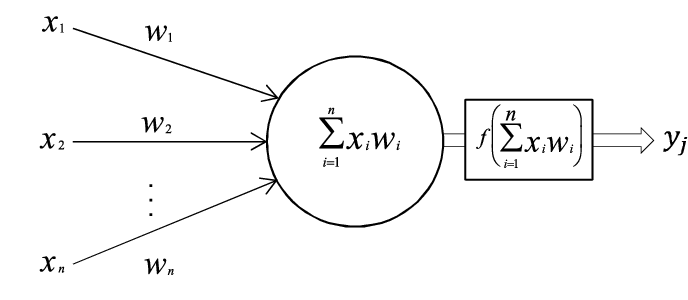
\includegraphics[scale=0.4]{one_node_NN.png}
	\caption{Interaction dynamics of the Agent and the Environment}
	\label{fig:diagram}
\end{figure}


Generally, NNs comprise multiple node layers through which data is passed, giving rise to what can be referred to as the depth of a neural network. In such networks, each layer of nodes trains on a distinct set of features based on the previous layer’s output. The further we move into the neural net, the more complex the features can be recognized by the nodes, since they aggregate and recombine features from the previous layer.

\begin{figure}[H] 
	\centering
	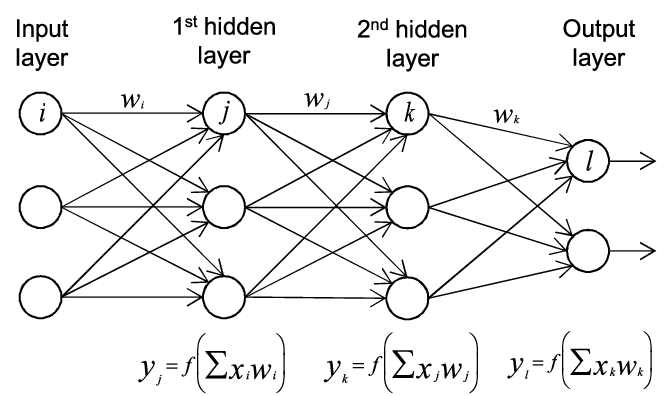
\includegraphics[scale=0.4]{feed-forward_NN.png}
	\caption{Interaction dynamics of the Agent and the Environment}
	\label{fig:diagram}
\end{figure}

The neural network used here takes the form $F^{\theta}: \mathbb{R}^d → (0,1)$ for $\theta \in \{\theta_0, \ldots, \theta_N  \}$, that is the parameters are trained via a neural network that outputs probabilities in the interval $(0,1)$. This is due to the fact that the G-B optimization algorithm is to be applied to a continuous function with respect to $\theta_n$, which $f^{\theta_n}$ is not. Hence, the multi-layer, feed-forward neural network takes the form:

\begin{equation}
F^{\theta}= \psi \circ a_3^{\theta} \circ \phi_{q_2} \circ a_2^{\theta} \circ \phi_{q_1} \circ a_1^{\theta}
\end{equation}
where 
\begin{itemize}
    \item $q_1, q_2$ are the number of nodes in the hidden layers
    \item $a_1^{\theta} : \mathbb{R}^d \rightarrow \mathbb{R}^{q_1}, a_2^{\theta}: \mathbb{R}^{q_1} \rightarrow \mathbb{R}^{q_2}$ are linear transformation functions: $a_i^{\theta}(x)=W_i x + b_i$ with matrices $W_1 \in \mathbb{R}^{q_1 \times d}, W_2 \in \mathbb{R}^{q_2 \times q_1}, W_3 \in \mathbb{R}^{q_2 \times 1}$ and vectors $b_1 \in \mathbb{R}^{q_1}, b_2 \in \mathbb{R}^{q_2}, b_3 \in \mathbb{R}^{1}$
    \item $\phi_{q_i}: \mathbb{R}^{q_i}$ is the ReLU activation function: $\phi_{q_1}(x_i, \ldots, x_{q_i})=(x_i^{+}, \ldots, x_{q_i}^{+})$
    \item $\psi = \mathbb{R} \rightarrow \mathbb{R}$ is the logistic sigmoid function: $\psi(x)=1/(1+ e^{-x})$.
\end{itemize}

Between the layers a batch normalization is also added, it takes the output from the previous layer and normalizes it before sending it to the next layer. This has the effect of stabilizing the neural network. 

The parameters will comprise $\theta = \{W_1, W_2,, W_3, b_1, b_2, b_3\}\in \mathbb{R}^q$, where $q=q_1(d+q_2+1)+2q_2+1$. The value of $d$ stands for the dimension, that is the number of assets and will be varied among $d=\{2,4, 5, 10, 20\}$. 


At each time step, for each epoch we compute $F^{\theta_n}$ using the $\theta_n$ from the previous epoch. Then, the parameter $\theta_n$ is update via backpropagation by the gradient of the loss function (Adam optimization algorithm \citep{kingma2014adam}), which is specified as:
\begin{equation}
    Loss = - \mathbb{E}[g(n, X_n)F^{\theta_n}(X_n) + g(\tau_{n+1}, X_{\tau_{n+1}})(1-F^{\theta_n}(X_n))]
\end{equation}
The aim is to determine $\theta_n \in \mathbb{R}^q$ so that the negative of the loss function is close to the supremum $\sup_{\theta \in \mathbb{R}^q}\mathbb{E}[g(n, X_n)F^{\theta}(X_n) + g(\tau_{n+1}, X_{\tau_{n+1}})(1-F^{\theta}(X_n))   ]$. From the stopping probabilities $F^{\theta_n}$, we retrieve $f^{\theta_n}$ as hard decisions $\{0,1  \}$. \\

We start with $f_N \equiv 1$ and proceed by backward induction for $n \in \{0, 1, \ldots, N-1 \}$. Once the parameters $\theta_n, \theta_{n+1}, \ldots, \theta_N \in \mathbb{R}^q$ have been found by SGD, we can compute the associated stopping time: 
\begin{equation}
\tau_{n+1} = \sum_{m=n+1}^N m f^{\theta_m}(X_m) \prod _{j=n+1}^{m-1} (1-f^{\theta_j}(X_j))
\end{equation}
which produces an expected value $\mathbb{E}g(\tau_{n+1}, X_{\tau_{n+1}})$ close to the optimum $V_{n+1}$. By simulating independent paths from the process $(X_n)_{n=0}^N)$ it is possible to derive a Monte Carlo estimate of the lower bound $L=\mathbb{E}g(\tau^{\Theta}, X_{\tau^{\Theta}})$ for the optimal value $V_0=\sup_{\tau \in \mathcal{T}}\mathbb{E}g(\tau, X_{\tau})$, given some assumptions on the hyperparameters and payoff function. 

\section{An application of the optimal switching problem}
Building upon the problem formulation presented by \cite{becker2019deep}, the optimal switching architecture will adopt the same probabilistic setup and similar assumptions as per being a finite-horizon discrete-time model pricing a Bermudan call option. Here we present an implementation of the switching problem with start and stop decision and derive a lower bound for the optimal value $V_0$. We will consider two versions:
\begin{itemize}
    \item a simpler version where we fix the final regime and proceed backwards along a single path
    \item a larger version where we follow two paths at the same time, differing in their final regime at maturity. At the moment, this second version is producing non-correct values.
\end{itemize}


\subsection{Training}

To approach the estimation of this iteration, we can start by providing a simulation of the process. For simplicity, we suppose a Bermudan max-call option expiring at time $T$ is written on $d$ assets, $\{X^i\}_{i=1}^d$, that gives the option holder the right to purchase one of the $d$ assets at strike price $K$ at any point in time on the time grid $0=t_0 > t_1> \ldots > t_N = T$, $t_n = n \cdot T/N$. We assume the following expression for the various cost and benefit:
\begin{itemize}
    \item Terminal function $\Gamma_i(N)$ is set to the option payoff. The terminal payoff is received at maturity, with no other costs nor payoffs
    \begin{equation}
    \begin{split}
    &\Gamma_0(N) = 0 \\
    &\Gamma_1(N) = \Big(\max_{i \in \{1, \ldots, d \}} x^i - K   \Big)^{+}
    \end{split}
    \end{equation}
    \item Running reward $\Psi_q = (\Psi_q(n))_{n \in \mathbb{N}}$ received while in mode $q \in \mathbb{I}$. 
    \begin{equation}
    \Psi_q(n) = \Big[\Big(\max_{d \in \{1, \ldots, D\}} x^i_n - K   \Big)^{+} \Big]
    \end{equation}
    \item Switching cost $\gamma_{i, j} = (\gamma_{i, j}(n))_{n \in \mathbb{N}}$ with $i,j \in \mathbb{I} = \{0, 1 \}$ represents the cost for switching from mode $i \in \mathbb{I}$ to mode $j \in \mathbb{I}$.
    \begin{equation}
    \begin{split}
    &\gamma_{0,0} \equiv \gamma_{1,1} \equiv 0 \\
    &\gamma_{0,1}(n) = \Big(\max_{d \in \{1, \ldots, D \}} x^i - K   \Big)^{+} + \delta,  \;\;\;\;\; \delta \sim \mathcal{N}(0,1)  \\ 
    &\gamma_{1, 0}(n) = -\Big(\max_{d \in \{1, \ldots, D \}} x^i - K   \Big)^{+} 
    \end{split}
    \end{equation}
\end{itemize}

We can introduce a discount factor $e^{- \rho t_n}$ and consider the discounted discrete-time optimal switching problem at time 0 starting in mode $i \in {0,1}$, defined as:

\begin{equation}
\begin{split}
    &J(\alpha; 0, i)= \mathbb{E} \Big[e^{- \rho T} \Gamma_{i}\mathbf{1}_{\{\tau_N \}} - \sum_{n \geq 1} e^{- \rho \tau_n (T/N)} \gamma_{\iota_{n-1}, \iota_n}(\tau_n) \mathbf{1}_{\{\tau_n < T \}} \Big]\\
    &V(i) = \sup_{\alpha \in \mathcal{A}_{0,1}} J(\alpha; 0,i)
\end{split}
\end{equation}

Now we can adjust the notation to follow more closely \cite{becker2019deep}'s notation. Since the option can be exercised only at $t_0, t_1, \ldots, t_N$, we can write the price as $\sup_{\alpha \in \mathcal{A}_{0,1}} \mathbb{E} g(\tau, X_{\tau}, i)$ where
\begin{equation}
    g(n, x, i) = e^{-\rho t_N}\Gamma_{i}\mathbf{1}_{\{\tau_N \}} - \sum_{t_n \geq 1} e^{- \rho t_n} \gamma_{\iota_{t_{n-1}}, \iota_{t_n}}(t_n) \mathbf{1}_{\{t_n < t_N \}}
\end{equation}
It is clear that this recursion requires to use, in case of a regime switch, the expected value of the value $Y$ at the new regime to which the process will be at the $n+1$ time step. 

Since $Y_0$ is deterministic, we can train the stopping times $\tau_1 \in \mathcal{T}_1$ as
\begin{equation}
    \tau_{1} = \sum_{n=1}^N n f^{\theta_n}(Y_n) \prod _{j=1}^{n-1} (1-f^{\theta_j}(Y_j))
\end{equation}
for $f^{\theta_N} \equiv 1$ and $f^{\theta_1}, \ldots, f^{\theta_{N-1}} : \mathbb{R}^{d+1} \rightarrow \{0,1\}$ given by the logit transform of $F^{\theta_n}$ with $\mathbb{I}=2$ and $q_1=q_2 = d+40$. The candidate optimal stopping time is 
\begin{equation}
\tau^{\Theta} = \begin{cases}
0 & \text{if } f_0=1\\
\tau_1 & \text{if } f_0=0
      
    \end{cases}
\end{equation}



\subsection{Parameters's optimization (Train)}
We simulate M paths of the process $(X_n)_{n=0}^N$ with dimension $d=1, \ldots, D$ and denote them by $(x_n^m)_{n=0}^N$ for $m=1, \ldots, M$ according to \ref{eq:eq1}:
\begin{equation}
    x_{n,d}^m = x_{0,i} \cdot \exp \Bigg\{ \sum_{k=0}^n \Big( (r-\delta_d - \sigma_d^2 /2) \Delta t + \sigma_d \sqrt{\Delta t} \cdpt Z_{k,d}^m   \Big) \Bigg\}
\end{equation}
where $\Delta t = T/N$ and $Z_{k,i}^m \sim \mathcal{N}(0,1)$. In addition we take the following hyperparameter values: $x_0^1=\{90, 100, 110\}; K=90;\sigma = 20; d=\{2, 4, 5, 10, 20\}; r= 5\%; T=3;N=9$.



At maturity $N$, we choose $\theta_N \in \mathbb{R}^q$ such that $f^{\theta_N}\equiv 1$. As we do not have information regarding at which regime the process is, we consider both possibilities, that is $Y_n^{0,1}$, this means that two processes $\{Y\}$ will be carried backward in time.

For $n \leq N-1$ we determine $\theta_n \in \mathbb{R}^q$ recursively. Suppose we are at time step $n$, so that we have already obtained $f^{\theta_{n +1}}, \ldots, f^{\thetah_N} $, we can compute the time $n+1$ optimal stopping time for each of the $m$ paths:
\begin{equation}
    \tilde{\tau}_{n+1}^m = \sum_{k=n+1}^N k f^{\theta_k}(x_n^m) \prod_{j=n+1}^{k-1}(1-f^{\theta_j}(x_j))
\end{equation}
Along path $m$, the realized reward is:
\begin{equation}
    r^m_n(\theta_n) = g(n, x_n^m, i)F^{\theta}(x_n^m)+g(\tilde{\tau}_{n+1}^m, x^m_{\tilde{\tau}^m_{n+1}}, i)
\end{equation}
Thus, for large $M$, we approximate the expected value with averages of Monte Carlo samples across paths:
\begin{equation}
    \frac{1}{M}\sum_{m=1}^M r_n^m(\theta_n)
\end{equation}
which is a smooth function with respect to $\theta$ a.e. by construction and it is the function we optimize via gradient descent with respect to $\theta_n$. Once the optimal $\theta_n$ are obtained, we can translate $F^{\theta_n}$ into $0-1$ switching decisions $f^{\theta_n}$ by setting $f^{\theta_n}=1$ if $F^{\theta_n} \geq 0.5$ and to $0$ otherwise. This step is repeated for $n=N-1, \ldots, 0$.

\smallskip

The challenges encountered so far regards the performance of the neural network in terms of the application of stochastic gradient descent. This issue regard both the implementation of the optimal switching exercise and the reproduction of the optimal stopping from \cite{becker2019deep}. By inspecting the loss curves generated at each time step, given that a NN is fitted for each $n=\{N-1, \ldots, 1\}$ time steps, it can be observed that the performance is poor. 

\begin{figure}[H] 
\centering
\begin{subfigure}{.5\textwidth}
  \centering
  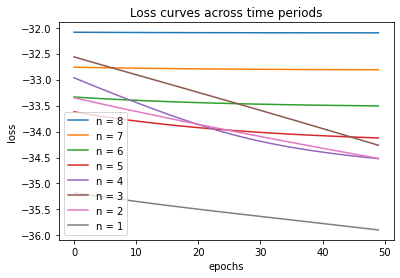
\includegraphics[width=.9\linewidth]{loss_curves_optStopping.png}
  \caption{Optimal Stopping}
  \label{fig:sub1}
\end{subfigure}%
\begin{subfigure}{.5\textwidth}
  \centering
  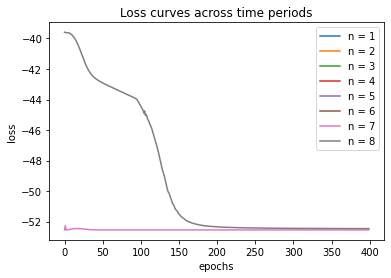
\includegraphics[width=.9\linewidth]{loss_curves_optSwitching.png}
  \caption{Optimal Switching}
  \label{fig:sub2}
\end{subfigure}
\caption{Loss curves (train) for 8 time steps}
\label{fig:test}
\end{figure}

In figure \ref{fig:test}, the loss curves for the optimal stopping seems to reveal that the NN is not learning the parameters and possibly underfitting. A similar event occurs in the optimal switching, combined with missing loss curves, due to failed backpropagation of gradients.

\subsection{Testing}
We now generate a new set of sample paths $(y_{n,i}^m)_{n=0}^N$ for $m=1, \ldots, M$. Using the parameters $\{\theta_n\}$ we have previously trained, for $n=N-1, \ldots, 0$, we compute
\begin{equation}
    \tilde{\tau}_{n+1}^m = \sum_{k=n+1}^N k f^{\theta_k}(y_k^m) \prod_{j=n+1}^{k-1}(1-f^{\theta_j}(y_j^m))
\end{equation}
for each sample path. At time $0$, the current optimal stopping time is given by 
\begin{equation}
    \tilde{\tau}_{0}^m = \sum_{n=1}^N k f^{\theta_n}(y_n^m) \prod_{k=1}^{n-1}(1-f^{\theta_k}(y_k^m))
\end{equation}
which estimates $\tau^{\Theta}$. The corresponding estimate of the expected value $\mathbb{E}g(\tau^{\Theta}, X_{\tau^{\Theta}})$ is given by
\begin{equation}
    \hat{V}=\frac{1}{M}\sum_{m=1}^M g(\tilde{\tau}, y_{\tilde{\tau}_m}^m, i)
\end{equation}
In the table \ref{table:opt_switch} below, some summary results of the estimated values with different initial values $X_0$ and dimensions $d$.
\begin{center}
\captionof{table}{Optimal switching estimated values}
\begin{tabular}{ |l|l|l|l| }
\hline
d  & $X_0$ & Lower bound & Time  \\
\hline \hline
2  & 90   & 97.339      & 0.009 \\
2  & 100  & 205.426     & 0.006 \\
2  & 110  & 315.878     & 0.007 \\
\hline
4  & 90   & 130.082     & 0.008 \\
4  & 100  & 235.951     & 0.008 \\
4  & 110  & 334.079     & 0.005 \\
\hline
5  & 90   & 134.486     & 0.008 \\
5  & 100  & 224.051     & 0.006 \\
5  & 110  & 282.737     & 0.006 \\
\hline
10 & 90   & 158.875     & 0.005 \\
10 & 100  & 273.452     & 0.008 \\
10 & 110  & 391.043     & 0.015 \\
\hline
20 & 90   & 100.447     & 0.008 \\
20 & 100  & 192.448     & 0.01  \\
20 & 110  & 301.107     & 0.009 \\

\hline

\end{tabular}
\label{table:opt_switch}
\end{center}


%--------------------------------------------------------------
\section{Github codes}
At the following \href{https://github.com/claudia-viaro/optimal_switching}{link}, there are implementations of the following algorithms:
\begin{itemize}
    \item Optimal stopping
    \item LSPI
    \item Optimal switching
\end{itemize}


%--------------------------------------------------------------
\newpage
\begin{appendices}
  \renewcommand\thetable{\thesection\arabic{table}}
  \renewcommand\thefigure{\thesection\arabic{figure}}

\section{Theorem}\label{section:appendix_d}
For a given $n \in \{ 0, 1, \ldots, N-1\}$, let $\tau_{n+1}$ be a stopping time in $\mathcal{T}_{n+1}$ of the form
\begin{equation}\label{theo}
    \tau_{n+1} = \sum_{m=n+1}^N m f_m(X_m) \prod_{j=n+1}^{m-1} (1-f_j(X_j))
\end{equation}
for measurable functions $f_{n+1}, \ldots, f_N : \mathbb{R}^d \rightarrow \{0,1\}$ with $f_N \equiv 1$. Then, there exists a measurable function $f_n: \mathbb{R}^d \rightarrow \{0,1\}$ such that $\tau_n \in \mathcal{T}_n$ satisfies 
\begin{equation}\label{eq13}
    \mathbb{R}g(\tau_n, X_{\tau_n}) \geq V_n - (V_{n+1}-\mathbb{E}g(\tau_{n+1}, X_{\tau_{n+1}})
\end{equation}
where $V_n$ and $V_{n+1}$ satisfy \ref{eq3}.
It follows that the overall optimal stopping time for \ref{eq1} is 
\begin{equation}\label{eq14}
    \tau = \sum_{n=1}^N n f_n(X_n) \prod_{k=0}^{n-1} (1-f_k(X_k))
\end{equation}





\end{appendices}



%--------------------------------------------------------------
\newpage
\bibliographystyle{agsm}
\bibliography{references_main}

\end{document}
